\section{Energy Ridges}
\label{al-energy-ridges}
The energy ridges between all the lowest energy \sap{1}s were calculated.
Two situations of particular interest arose.
The first was the discovery of intermediate \sap{1}s, while the second concerned the HTST reaction rate, its accuracy and efforts to improve it.

\subsubsection{Intermediate \sap{1}s}
\begin{figure}[hp]
\begin{center}
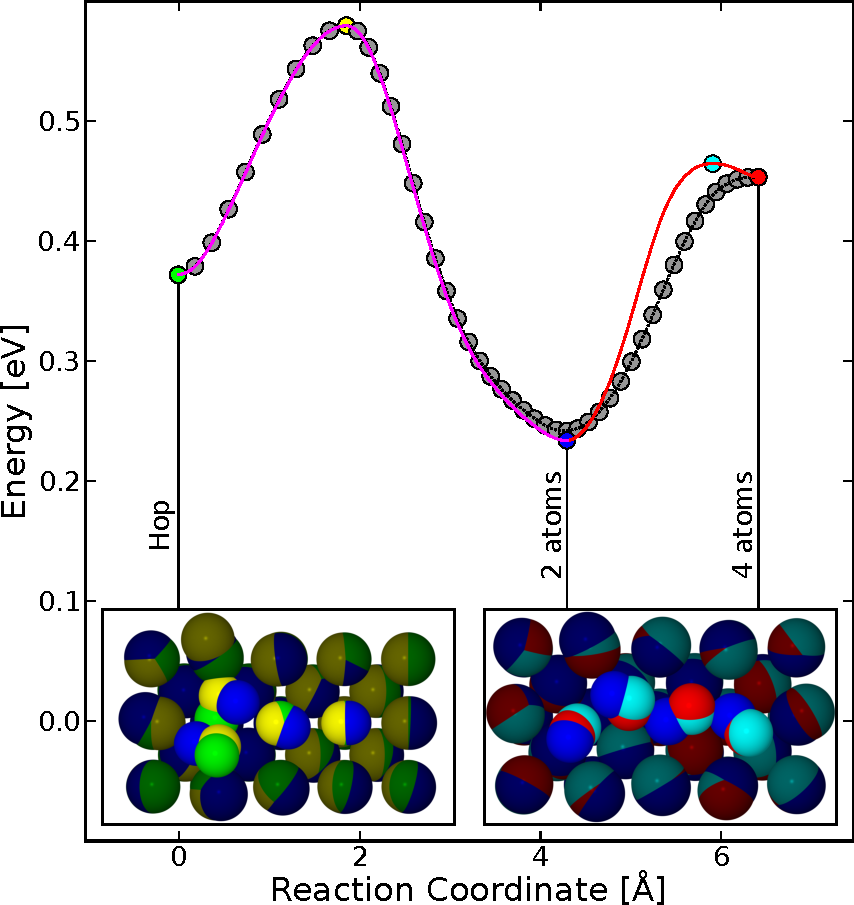
\includegraphics[width = 1.0\linewidth]{discovery}
    \parbox{0.85\linewidth}{
\caption{
Calculated path at the ridge between the \sap{1}s for a hop and concerted 4-atom displacement.
The circles show the position of converged images (coloured circles for \sap{1}s and \sap{2}s, but grey for the rest). 
These \sap{1}s turned out not to be adjacent on a ridge and the path optimisation reveals an intermediate \sap{1}, the one for the concerted 2-atom displacement.
The full path is not able to accurately locate the intermediate \sap{1} and the lower energy \sap{2} due to finite resolution in the discretisation and corner-cutting (grey circles)
The exact configuration of the \sap{1} can be found using a \sap{1} finding algorithm starting with the approximation obtained from the optimised path.
Then, a calculation of a shorter path (red line), between the \sap{1}s of the 2-atom and 4-atom displacements, locates the intermediate \sap{2} accurately (cyan circle)
The insets show an overlay of three configurations, two adjacent \sap{1}s and the intermediate \sap{2}.
The atom colours correspond to the coloured spheres of the energy ridge.
}
\label{fig:discovery}
}
\end{center}
\end{figure}

As can be seen in \fref{fig:discovery} there is a significant energy ridge "barrier" separating the hop and concerted 2 atom \sap{1}s.
More interestingly, ridge calculations between the more populous concerted \sap{1}s (3 and 4 atom) and the hop revealed that they were interspersed with the concerted 2 atom \sap{1}.
This is not surprising as the concerted mechanisms are all quite similar with regards to their coordinates, while the hop mechanism is inherently different, as can be seen in insets of figures \ref{fig:discovery} and \ref{fig:low-barriers}.

Finding the intermediate \sap{1} is only accurate in the limit of an infinite amount of images and no corner cutting, but the lowest energy image gives a good starting guess, both for the coordinates and the minimum mode, for traditional \sap{1} methods, such as the Dimer.
It would be possible to implement a "sinking" image alteration of the effective force in a manner similar to the climbing image but this was not done here.
Similarly, corner cutting prevents rigorous convergence to the lower energy \sap{2}.
A second climbing image would converge exactly to this point but this was not done.\footnote{Implementing multiple climbing or sinking images is in principle not difficult but the ramifications could be dire, e.g. in systems with rugged landscapes and a limited amount of images.}
However, performing a second ridge calculation with the intermediate \sap{1}(s) as end points yields the exact \sap{1} and, apart from the possible corner cutting, the ridge.
These latter paths are displayed as red curves in \fref{fig:discovery}

\subsubsection{Beyond Harmonicity}
\begin{figure}[hp]
\begin{center}
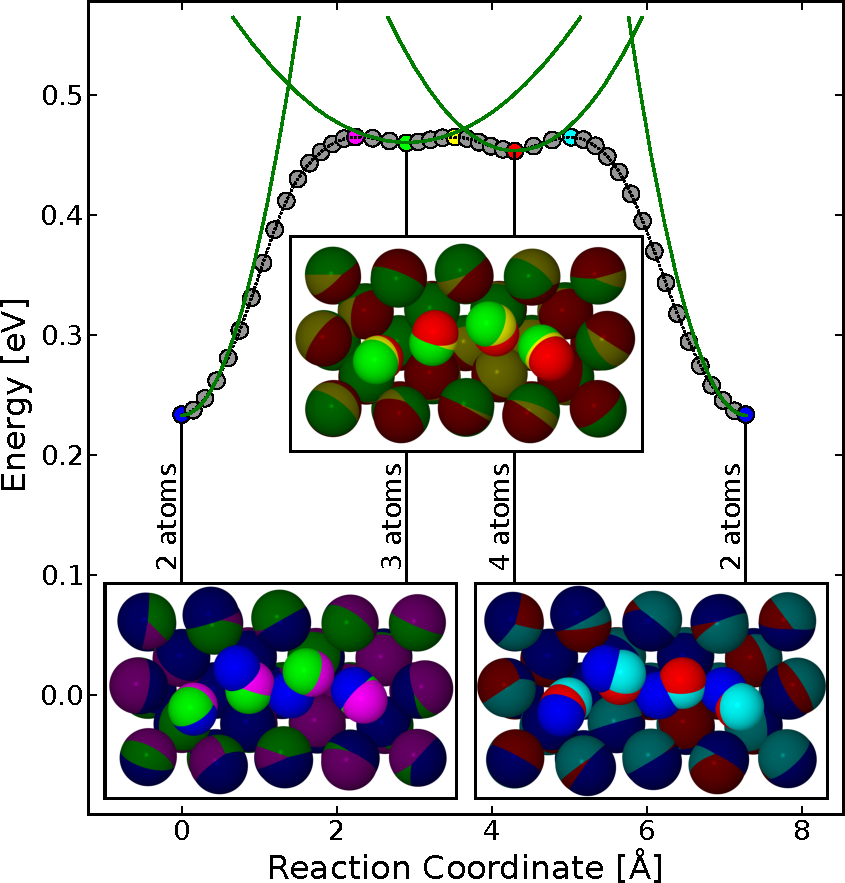
\includegraphics[width = 1.0\linewidth]{low-barriers}
    \parbox{0.85\linewidth}{
\caption{
The energy ridge going through \sap{1}s of 2-atom, 3-atom, 4-atom and, then the same, 2-atom concerted displacement.
The circles represent the position of images in the optimised paths, the \sap{1}s and the \sap{2}s being coloured differently but the rest coloured grey.
The green curves represent harmonic approximations to the energy surface at each \sap{1}.
The insets show an overlay of three configurations, two adjacent \sap{1}s and the intermediate \sap{2}.
The atom colours correspond to the coloured spheres of the energy ridge.
}
\label{fig:low-barriers}
}
\end{center}
\end{figure}

\begin{SCfigure}[5.0][h]
\centering
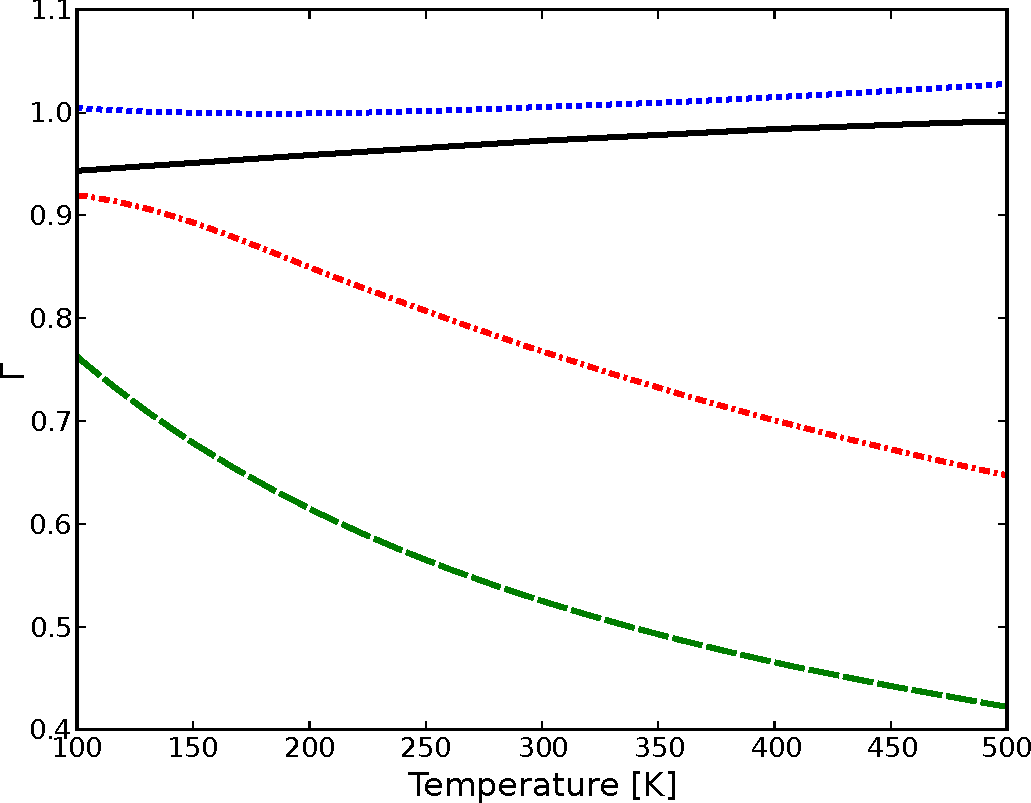
\includegraphics[width = 0.45\linewidth]{integral-ratios}
\caption{
The harmonic correction ratio, $\Gamma$, defined in \fref{eq:htst-correction-factor},
between the configuration integrals of the potential energy ridge shown in \fref{fig:low-barriers} and the corresponding harmonic approximations.
The lines represent the ratio for individual processes: concerted 2 atom (blue, dotted), 3 atom (green, dashed), 4 atom (red, dash-dotted) and the combined ratio for all the processes combined (black, solid).
For the individual processes, the end points of the ridge integral are the adjacent \sap{2}s, while the full integral is done for the whole ridge.
}
\label{fig:integral-ratios}
\end{SCfigure}

The ridges between the, similar, concerted motion \sap{1}s are shown in \fref{fig:low-barriers}.
It can be clearly seen that applying HTST to the concerted 3 and 4 atom \sap{1}s is highly questionable as their neighbouring \sap{2}s are very low, $\mytilde 0.005\unit{eV}$ and $0.012\unit{eV}$, certainly lower than the $5\kB T$ rule of thumb\footnote{at any temperature above $9\unit{K}$ and $28\unit{K}$ respectively.}.
However, applying HTST to the concerted 2 atom mechanism is more justified, by visual inspection the ridge is fairly near harmonicity up to the $5\kB T = 0.128\unit{eV}$ limit at room temperature and the \sap{2}s are still higher.
\Fref{fig:integral-ratios} further shows that the concerted 2 atom rate has a correction factor, $\Gamma$, of approximately $1.0$ throughout the temperature range while the concerted 3 and 4 atom mechanisms have significant correction factors at all temperatures.

It might appear wise to rigorously calculate such a correction factor for all the degrees of freedom until one considers the complexity of such an exercise.
Figure 6 in paper \ref{pap:second-order} makes an effort to put into context the abundance of ridges on which each \sap{1} lies but, of course, fails to do so properly due to the immense dimensionality (771 degrees of freedom) of the PES.
Not only finding all the \sap{1}s leading out of a given basin but also finding all neighbouring \sap{2}s and ridges for each one would be folly due to the sheer amount of possible \sap{}s.
Furthermore, as stated when introducing the correction factor (\fref{eq:htst-correction-factor}), $\Gamma$ is not a rigorous correction factor and should not be used as such.
However, using the ridge to calculate a more precise reaction rate, outside the HTST framework, seems appropriate and will make an interesting subject for future research.
